\begin{figure}[h]
  \centering
  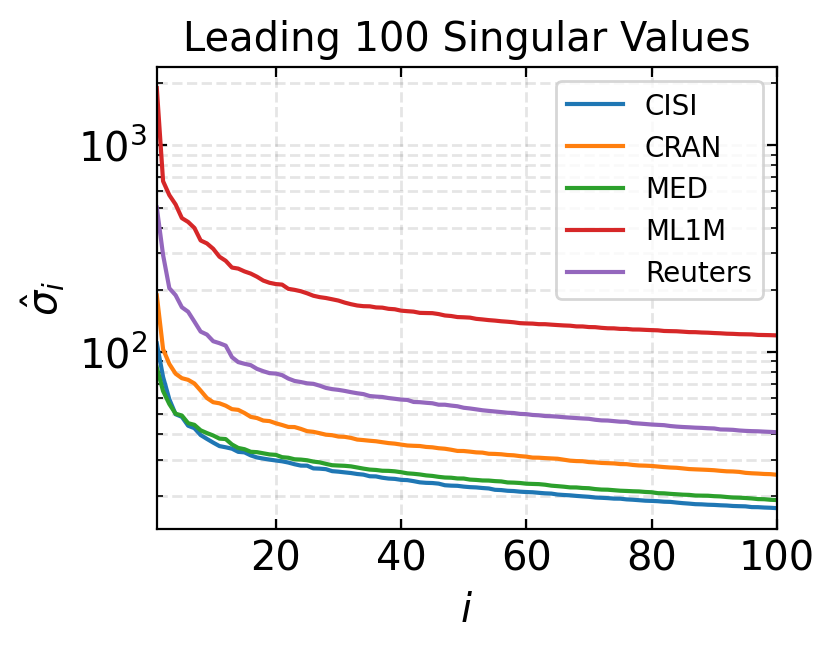
\includegraphics[width=0.7\textwidth]{../openreview/figures/sv_100_profile.png}
  \captionof{figure}{Leading 100 singular values for each dataset.}
  \label{fig:sv}
\end{figure}

\begin{table}[h]
  \centering
  \begin{tabular}{cccc}
    \toprule
    Dataset       & Rows  & Columns & nnz(A)/row \\
    \midrule
    CISI \cite{LSISite}                                     & 5609  &    1460 &      12.17 \\
    CRAN \cite{LSISite}                                     & 4612  &    1398 &      18.06 \\
    MED  \cite{LSISite}                                     & 5831  &    1033 &       8.92 \\
    ML1M \cite{Harper2015}                                  & 6040  &    3952 &     165.60 \\
    Reuters-21578 \cite{Cai2005, Cai2007, Cai2008, Cai2009} & 18933 &    8293 &      20.57 \\
    \bottomrule
  \end{tabular}
  \captionof{table}{Number of rows, columns, and average non-zero elements in each row for datasets.}
  \label{table:datasets}
\end{table}
